\documentclass{article}


% if you need to pass options to natbib, use, e.g.:
%     \PassOptionsToPackage{numbers, compress}{natbib}
% before loading neurips_2023


% ready for submission
\usepackage[final]{neurips_2023}


% to compile a preprint version, e.g., for submission to arXiv, add add the
% [preprint] option:
%     \usepackage[preprint]{neurips_2023}


% to compile a camera-ready version, add the [final] option, e.g.:
%     \usepackage[final]{neurips_2023}


% to avoid loading the natbib package, add option nonatbib:
%    \usepackage[nonatbib]{neurips_2023}


\usepackage[utf8]{inputenc} % allow utf-8 input
\usepackage[T1]{fontenc}    % use 8-bit T1 fonts
\usepackage{hyperref}       % hyperlinks
\usepackage{url}            % simple URL typesetting
\usepackage{booktabs}       % professional-quality tables
\usepackage{amsmath, amssymb, amsthm, amsfonts}       % blackboard math symbols
\usepackage{nicefrac}       % compact symbols for 1/2, etc.
\usepackage{microtype}      % microtypography
\usepackage{xcolor}         % colors
\usepackage{array}
\usepackage{graphicx}
\usepackage{caption}

\title{Is the Linear Correlation Between Classification and Rotation/Jigsaw Prediction Model-Invariant?}


% The \author macro works with any number of authors. There are two commands
% used to separate the names and addresses of multiple authors: \And and \AND.
%
% Using \And between authors leaves it to LaTeX to determine where to break the
% lines. Using \AND forces a line break at that point. So, if LaTeX puts 3 of 4
% authors names on the first line, and the last on the second line, try using
% \AND instead of \And before the third author name.


\author{%
  Callum Koh\\
  College of Engineering, Computing and Cybernetics\\
  Australian National University\\
  Canberra ACT 2601, Australia \\
  \texttt{u7122029@anu.edu.au} \\
  % examples of more authors
  % \And
  % Coauthor \\
  % Affiliation \\
  % Address \\
  % \texttt{email} \\
  % \AND
  % Coauthor \\
  % Affiliation \\
  % Address \\
  % \texttt{email} \\
  % \And
  % Coauthor \\
  % Affiliation \\
  % Address \\
  % \texttt{email} \\
  % \And
  % Coauthor \\
  % Affiliation \\
  % Address \\
  % \texttt{email} \\
}

\setlength\extrarowheight{3pt}

\begin{document}


\maketitle


\begin{abstract}
We verify the linear relationship between image classification accuracy (classification) and rotation prediction (rotation) over the CIFAR-10 dataset and its variants. This extends previous work where the same correlation was observed over numerous datasets but one fixed classifier. We also verify the linear correlation for classification and jigsaw solving accuracy (jigsaw) over the same dataset. For both comparisons, all models (except one) showed a strong correlation over datasets constructed by directly using image transformations ($R^2 > 0.71$ for classification vs. rotation, $R^2 > 0.61$ for classification vs. jigsaw). However, some models showed a weak linear correlation between classification and rotation/jigsaw accuracy on images outside of CIFAR-10. This suggests that estimating a model's classification accuracy based on rotation/jigsaw accuracy depends on the model itself, however, this must be investigated further.
\end{abstract}

\section{Introduction}
Generally, image classification models are extensively trained to achive optimal accuracy on a training dataset and a validation dataset \cite{dridi2021supervised, nasteski2017overview}. Both datasets only cover a small subset of all possible scenarios encounterable in the real world \cite{gopalan2011domain}. This means that no matter how optimally a model for recognising road edges is trained for any imaginable scenario, there will eventually come a case where it will perform poorly. It is hence imperative that the performance of the classifier is closely monitored when used in the real world. Unfortunately, the images fed into a model outside the training environment are unlabeled. So it is impossible to measure model accuracy without manually adding labels to each image - which is a repetitive, time-consuming task. However, it has been previously shown that a classifier's accuracy can be estimated through its performance on rotation prediction and jigsaw solving \cite{Deng:ICML2021}. Current findings have observed this correlation for some datasets such as CIFAR-10 \cite{krizhevsky2009learning}, ImageNet \cite{deng2009imagenet}, COCO \cite{cocodataset} and MNIST \cite{deng2012mnist}, but each only had a few classifiers each to show it. Our work keeps the dataset fixed to CIFAR-10, and we use many different classifiers of varying complexity to verify if the linear correlation of classification vs rotation and classification vs jigsaw are maintained across all of them.

\section{Related Work}
\paragraph{Image Classification} This task involves predicting the contents of an image. For example, a classifier can be trained to identify cars in an image. It is a core task that allows - among many other things - self-driving cars to travel safely \cite{du2019self, kulkarni2018traffic, kuehnle1998winter}, quality control machines to flag defective products \cite{kunkel2020quality}, specialised computers to read even the messiest handwritten addresses on envelopes \cite{gilloux1993research}, and hospital devices to recognise various lung diseases through x-rays \cite{abbas2021classification, wang2017chestx}. It is difficult to deny that over the last 20 years, research in this field has rapidly grown due to its wide range of applications and its potential to mimic human accuracy in this field \cite{singh2020image}.

\paragraph{Rotation Prediction} This is a task where a model must predict the canonical orientation of an image \cite{8932427}. It can help with determining the slant of a surface from an image \cite{413886}, stabilising shaky footage from a video recording or livestream \cite{fischer2015image}, determining the image transformations applied to an image \cite{gidaris2018unsupervised}, and many more applications. In the past, the canonical orientation was handled over a discrete set of possible rotations, such as $0^\circ$, $90^\circ$, $180^\circ$ and $270^\circ$ when determining the upright appearance of a scanned document \cite{fischer2015image}. Today, canonical orientations can be determined over the interval $[0^\circ, 360^\circ)$ of rotational angles \cite{fischer2015image, 8932427}.

\paragraph{Jigsaw Solving.} This is a task where a model must predict the canonical arrangement of an image that has been divided into an $n$ by $n$ grid of equally-sized portions and positionally shuffled. Some works have trained models on image classification alongside jigsaw solving to improve its performance on data outside the training environment \cite{noroozi2016unsupervised}. By combining the losses together for backpropagation, the jigsaw task can be loosely viewed as a form of regularisation to avoid overfitting. Training models to solve jigsaw puzzles has also been a strategy for performing object reconstruction, which is useful for archeologists \cite{8451094}.

\section{Method}
\begin{figure}[!t]
  \centering
  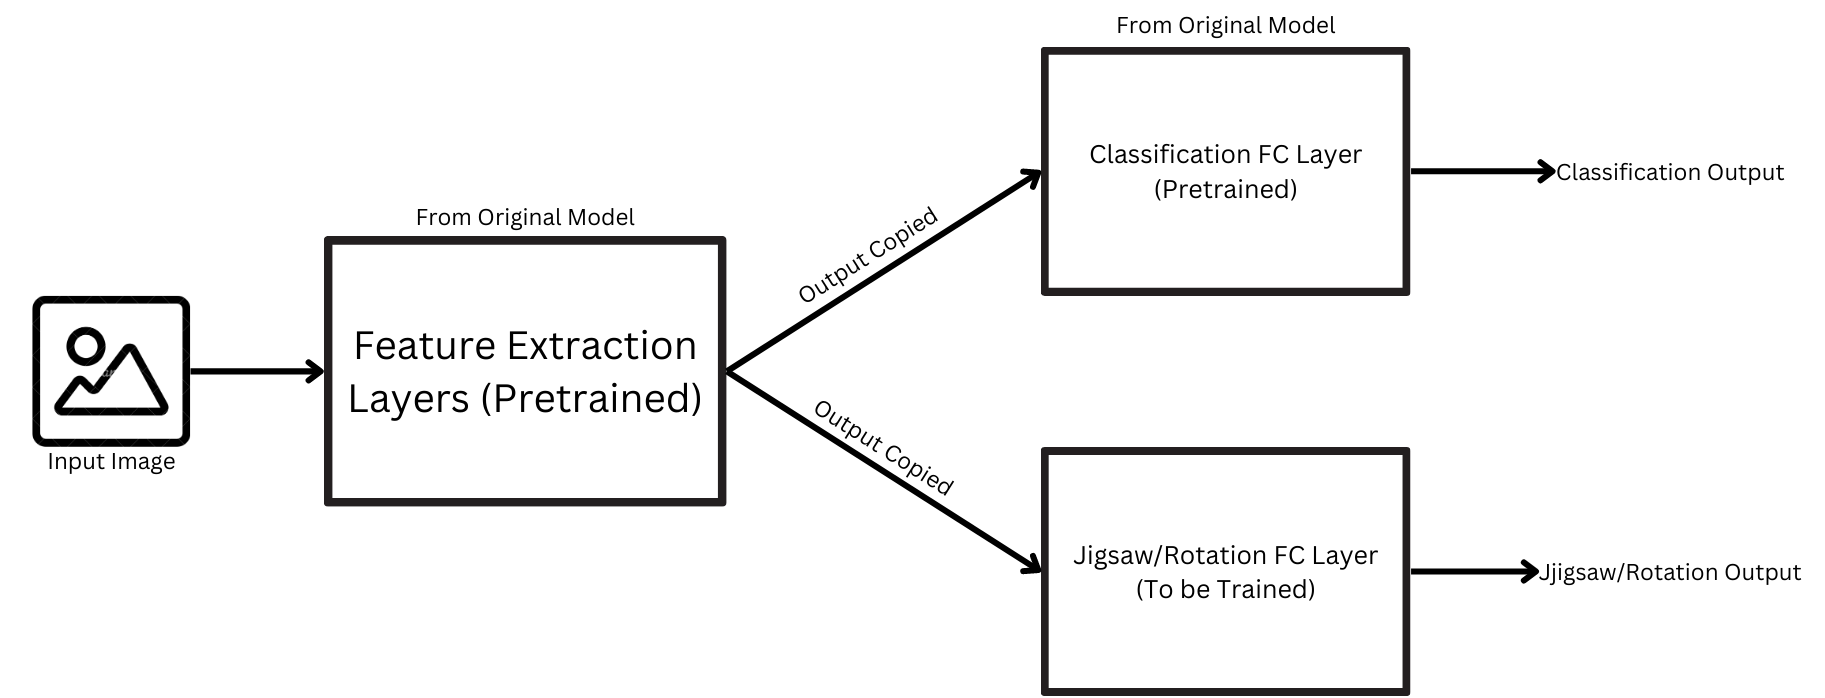
\includegraphics[scale=0.2]{images/diagram.png}
  \caption{Model Setup for Image Classification and Jigsaw Solving}\label{fig:method}
\end{figure}
\subsection{Definitions} 
Let $D_\text{src}^{(i)} = \{(X_{\text{src}, k}^{(i)}, y_{\text{sre}, k}^{(i)})\}_{k = 1}^{n_i}$ be the $i$-th dataset from a particular source src, where $n_i$ is the number of images, $X_{\text{src}, k}^{(i)}$ is the $k$-th image from the dataset, and $y_{\text{sre}, k}^{(i)}$ is the corresponding label. If there is only one dataset from the given source, the $(i)$ will be omitted. For example, there is only one training dataset $D_\text{train}$ and one testing dataset $D_\text{test}$ in CIFAR-10.

Now let $C_\text{sre} = \{D_{\text{sre}}^{(i)}\}^{m_\text{src}}_{i = 1}$ be a collection of $m_\text{src} \in \mathbb{N}$ datasets from a particular source. We call this set a domain, and in our work we consider the interior domain $C_\text{int}$ and the exterior domain $C_\text{ext}$. The interior domain refers to the datasets that are obtained through a series of image transformations applied to all images \textit{inside} $D_\text{test}$. The exterior domain refers to datasets constructed using images \textit{outside} $D_\text{train}$ and $D_\text{test}$. The images constructing these datasets can be obtained through Google Image Search, Instagram, or other places. They can also be obtained through image transformations of these pictures.

\subsection{Estimating Classifier Accuracy}
From here, our aim is to take a pretrained image classification model $M$ and test its performance on classifying images, jigsaw solving and rotation prediction over $C_\text{int}$ and $C_\text{ext}$. To do so we divide $M$ into two mutually exclusive parts: the classification layer $CL$ which is usually the last fully connected layer in $M$, and the feature extraction layers $FE$ - everything else in $M$. We then perform the following steps:
\begin{enumerate}
  \item Keep the weights and biases of $FE$ and $CL$ constant.
  \item Introduce a new fully connected layer $SSL$ for a self-supervised task that has the same dimensions as $CL$ but with output size matching the requirements of the self-supervised task. This layer will take the output of $FE$ as input.
  \item Train $M$ on the self-supervised task using data from $D_\text{train}$ and $D_\text{test}$, using the output of $SSL$ to evaluate performance.
  \item Evaluate the classification accuracy of $M$ over $C_\text{int}$ using the output of $CL$,
  \item Evaluate the accuracy of $M$ on the self-supervised task over $C_\text{int}$ using the output of $SSL$,
  \item Repeat steps 4 and 5 using $C_\text{ext}$ instead,
  \item Make a scatter plot of classification accuracy vs self-supervised task accuracy over $C_\text{int}$,
  \item Fit a linear regression model to the scatter plot,
  \item Repeat the previous step with $C_\text{ext}$.
  \item Repeat all steps in order for another classifier.
\end{enumerate}
Here, the words "self-supervised task" refer to either rotation prediction or jigsaw solving. Figure \ref{fig:method} illustrates the setup for testing a model for jigsaw solving. For rotation prediction, we simply change the number of output features in the Jigsaw permutation layer to match the number of output classes.

\paragraph{Linear Correlation Strength} For each classifier we evaluate the fit of the linear regression model on classification vs. rotation and classification vs. jigsaw using the Root Mean Square Error (RMSE) to determine the average deviation of each dataset from the line \cite{chai2014root}. We also use the Coefficient of Determination ($R^2$) to determine how much variation can be explained by the linear model \cite{nagelkerke1991note}.
\subsection{Datasets}
In our work, the interior domain $C_\text{int}$ contains 1000 datasets, each of which have modified images from $D_\text{test}$ via combinations of image transformations. The specifics are further described in \cite{deng2021labels}. 

The exterior domain contains 40 datasets. One of these datasets was the CIFAR10.1 dataset \cite{recht2018cifar10.1, torralba2008tinyimages}, composed of 2000 images with the same labels as CIFAR-10 but are not part of CIFAR-10. Its original purpose was to understand the performance of classifiers trained on CIFAR-10 when given unseen data with the same labels. 19 datasets come from CIFAR-10.1-C \cite{hendrycks2019robustness}, each of which are modified versions of CIFAR-10.1 by applying a series of image transformations. The remaining 20 datasets are from CIFAR-10-F, which each contain images from the same distribution as CIFAR-10, but are from Flickr.

\subsection{Self-Supervised Layer Training}
Since all the image classification models we have chosen are pretrained, and their weights and biases are kept constant, we can say for sure that any loss function we use for this task will also remain constant. In turn, the accuracy of the model over a fixed dataset will remain unchanged over the training process. Consequently, we can ignore image classification loss. 

\paragraph{Rotation Prediction} Let $f_\text{FE}$ be a function that applies the feature extraction layer of a model on an image, and $f_\text{R}$ be the function that applies the rotation prediction layer to a feature vector. If $\mathcal{L}_\text{CE}$ is the cross-entropy loss function, then the loss function for rotation prediction over a dataset $D_\text{src}$ can be written as
\begin{equation}
  \mathcal{L}_\text{R}(D_\text{src}) = \frac{1}{n_\text{src}}\sum_{k = 1}^{n_\text{src}} \mathcal{L}_\text{CE}(y_{\text{src}, k}, f_\text{R}(f_\text{FE}(X_{\text{src}, k})))
\end{equation}
 %When training the model on rotation prediction, we feed in an image $X_{\text{train}, model}$ from $D_\text{train}$ that has been rotated about its centre at an angle of $\theta \in \{0^\circ,180^\circ,270^\circ\}$ into the model by applying the feature extraction layer $f_\text{FE}$ to obtain the feature vector, then applying the rotation prediction function $f_\text{R}$ to obtain a .

\paragraph{Jigsaw Solving} We can write the loss function here in a similar manner, with $f_\text{J}$ being the function that applies the jigsaw prediction layer to a feature vector.
\begin{equation}
  \mathcal{L}_\text{J}(D_\text{src}) = \frac{1}{n_\text{src}}\sum_{k = 1}^{n_\text{src}} \mathcal{L}_\text{CE}(y_{\text{src}, k}, f_\text{J}(f_\text{FE}(X_{\text{src}, k})))
\end{equation}

For both tasks, we train each model for a maximum of 25 epochs over $D_\text{train}$ with learning rate 1e-2, weight decay 1e-4, and momentum 0.9. We save the model that achieved the highest self-supervised task accuracy on $D_\text{test}$ for evaluating the same task over $C_\text{int}$ and $C_\text{ext}$. All implementation details can be found in the GitHub repository \cite{Koh-u7122029-autoeval-baselines}.

\subsection{Selected Classifiers}\label{sec:sc}
\begin{figure}[!t]
  \minipage{0.5\textwidth}
    \includegraphics[width=\linewidth]{images/resnet1202_rot_int.png}
    \caption*{(a)}
  \endminipage\hfill
  \minipage{0.5\textwidth}
    \includegraphics[width=\linewidth]{images/resnet1202_rot_ext.png}
    \caption*{(b)}
  \endminipage
  \vfill
  \minipage{0.5\textwidth}
    \includegraphics[width=\linewidth]{images/resnet1202_jig_int.png}
    \caption*{(c)}
  \endminipage\hfill
  \minipage{0.5\textwidth}
    \includegraphics[width=\linewidth]{images/resnet1202_jig_ext.png}
    \caption*{(d)}
  \endminipage
  \caption{Classification vs. Rotation/Jigsaw for the ResNet1202 Model.}\label{fig:samples}
\end{figure}
We train a total of 17 classifiers on rotation prediction and jigsaw solving, and we briefly introduce them here in decreasing order of complexity, according to the general number of parameters in the models from PyTorch's no\_parameters method \cite{NEURIPS2019_9015}.
\paragraph{ResNet} ResNet was developed by He et al. to address the vanishing gradient problem when deep neural networks were being trained on a given task \cite{DBLP:journals/corr/HeZRS15}. The architecture of ResNet has many forms, each of which are mostly dependent on the number of layers. ResNet-152 for instance contains 152 layers. In our work we use ResNet-20, ResNet-32, ResNet-44, ResNet-56 whose pretrained weights were obtained from \cite{Chen-pytorch-cifar-models}. We also use ResNet-110 and ResNet-1202, whose weights can be obtained from \cite{Koh-pytorch-resnet-cifar10} which is a forked repository of \cite{Idelbayev18a}.

\paragraph{MobileNetV2} MobileNetV2 was developed to be accurate at classifying images while minimising power consumption and latency on mobile devices \cite{DBLP:journals/corr/abs-1905-02244}. We obtained the pretrained weights from \cite{Chen-pytorch-cifar-models}.

\paragraph{InceptionV3} InceptionV3 was developed by Google and was designed to be a deep convolutional network while preventing the number of parameters from becoming too numerous \cite{DBLP:journals/corr/SzegedyVISW15}. It achieved a 79.8\% classification accuracy on the ImageNet dataset.

\paragraph{RepVGG} RepVGG is a convolutional neural network that takes inspiration from VGG. Its architecture during training reminisces that of ResNet, but uses 1 by 1 branches during training only. During inference, the model only uses 3 by 3 convolutional layers and ReLU layers \cite{DBLP:journals/corr/abs-2101-03697}. It achieved over 80\% top-1 accuracy over the ImageNet dataset and is much more efficient than models such as ResNet-101.

\paragraph{DenseNet} We use three versions of DenseNet, namely DenseNet-121, DenseNet-161 and DenseNet-169. DenseNet was designed with grouped layers called dense blocks, whose later layers take in features outputted from all previous layers. This addresses the vanishing gradient problem similarly to ResNet \cite{DBLP:journals/corr/HuangLW16a}.

\paragraph{ShuffleNet} Is an extremely efficient convolutional neural network designed for use on mobile devices with computing speeds of 10 to 150 MFLOPS while achieving accuracies similar to that of AlexNet. Consequently, ShuffleNet runs around 13 times faster than AlexNet \cite{DBLP:journals/corr/ZhangZLS17}.

\paragraph{AlexNet} Is a convolutional neural network proposed by Krizhevsky et al. that won the LSVRC competition in 2012 \cite{krizhevsky2017imagenet}. It was one of the first networks that inspired the use of convolutional layers in later models such as ResNet, however, its performance has evidently been well and truly surpassed by all the models mentioned earlier. From this point forward, the models we introduce will become less and less complex to approximately find the minimum model complexity required to show the aforementioned linear correlation.

\paragraph{LeNet5} Is a convolutional neural network proposed by LeCun et al in 1998 to recognise grayscale handwritten digits in the MNIST dataset \cite{726791}. The model has been adapted to accept RGB images from the CIFAR-10 dataset.

\paragraph{Linear Classification} This model has a feature extraction layer that flattens the image into a $(32\cdot 32 \cdot 3) \times 1$ vector before passing it into a fully connected layer which will determine the model's prediction. It essentially tries to fit a linear model to $D_\text{train}$ for all tasks even though we know fully well that the classes of each task is not linearly seperable. We are unsure if the name "Linear Classification" is the original name for this model, however, the general concept of fitting a line to a given dataset has existed for centuries in the hopes of mathematically formalising the linear relationship between a collection of variables \cite{Belov2018}.

\paragraph{One Braincell Model (OBC)} This model takes an image, and takes the arithmetic mean of all pixel intensities of all channels to output a scalar. This scalar is then passed into the fully-connected layer which will output the model's prediction for the given task. We called this model the One Braincell (OBC) model due to the sheer simplicity of this model, how poorly we expected it to perform on all tasks, and how its feature extraction layer gives an analogous amount of data to the classification layer as what a single neuron in the brain gives to the prefrontal cortex. Just like the linear classification model, we are unsure if there have been other names attributed to this model.

\section{Results}
For the sake of brevity, we present our results for a subset of all tested models.
\subsection{Classification vs. Rotation Accuracy}
All results for this section can be found in Table \ref{tbl:cavra}.
\begin{table}[t]
  \centering
  \caption{Classification Accuracy vs. Rotation Accuracy for selected models.}\label{tbl:cavra}
  \begin{tabular}{llllllll}
  \cline{1-8}
  \multicolumn{2}{c}{}           & \multicolumn{2}{c}{Int. Dom}     & \multicolumn{2}{c}{Ext. Dom}          & \multicolumn{2}{c}{Ext. Dom w/ Int. Dom Fit}            \\ \hline
  Model & No. Params & $R^2$ & RSME & $R^2$ & RSME & $R^2$ & RSME \\ \hline
  ResNet1202   &   3605   &  0.956  &   2.775   &    0.636     &   6.493   &    0.495      &   7.655   \\ 
  DenseNet169   &   508   &  0.934  &   5.255   &    0.726     &   5.408   &    0.062      &   10.00   \\ 
  DenseNet121   &   364   &  0.976  &   3.070   &    0.757     &   4.835   &    0.584      &   6.333   \\ 
  InceptionV3   &   272   &  0.820  &   8.479   &    0.347     &   8.657   &    0.175      &   9.730   \\ 
  MobileNetV2   &   158   &  0.927  &   4.603   &    0.734     &   6.884   &    0.519      &   9.252   \\ 
  AlexNet       &    16   &  0.761  &   4.211   &    0.757     &   2.851   &    0.727      &   2.955   \\ 
  LeNet5        &    14   &  0.719  &   4.457   &    0.004     &   4.922   &    -0.481     &   6.002   \\ 
  Linear        &     2   &  0.765  &   2.901   &    0.216     &   3.330   &    -1.312     &   5.717   \\ \hline
  \end{tabular}
\end{table}
\paragraph{Interior Domain} We observe that the $R^2$ score for all models in the interior domain (except for OBC, which we will discuss later) is over 0.71. DenseNet121 scored the highest at 0.97. This means that for a fixed model, at least 71\% of the variation between classification accuracy and rotation accuracy can be explained by the line of best fit for this model. Consequently, there is a strong linear correlation between the two variables over the interior domain and for almost any model. The RMSE for all selected models is below 8.657 for all models, which implies that the general spread of the data from the line is not too large. We can also see that there appears to be a general correlation between the number of model parameters and the $R^2$ coefficient. 

\paragraph{Exterior Domain} We observe that for each model, the linear regression fitted on the interior domain does not necessarily fit the exterior domain. The strength of the correlation is either weak - represented by $R^2 \in [0, 0.45]$ - or inappropriate, represented by $R^2 < 0$. Furthermore, we can see that although AlexNet showed that the linear model fitted on the interior domain is also a good fit for the exterior domain, the same cannot be said for LeNet5. Although both models were designed differently, their number of parameters suggest that they are of similar complexity, and hence we cannot estimate classification accuracy based on the linear model from the interior domain. Our results for InceptionV3 also agree with this claim, as although it has a high $R^2 = 0.820$ on the interior domain, the same linear model fitted on the exterior domain showed a very weak correlation of $0.175$. On the other hand, if we fit an entirely new linear model to the exterior domain results for each model, we observe that the simplest ones including LeNet5, Linear, and OBC had the lowest $R^2$ scores, however, we did not expect InceptionV3, a model that has nearly twice the number of parameters as MobileNetV2 to give an $R^2$ that is half as strong. Every other model tested had medium to strong correlations, agreeing with the work of Deng et al. \cite{Deng:ICML2021}. Subfigures (a) and (b) of Figure \ref{fig:samples} show the linear model fitted to the performance of ResNet1202 over image classification vs rotation/jigsaw accuracy. Each datapoint represents a dataset from the respective domain. We can see that interior domain line is not the best representeation of the exterior domain results ($R^2 = 0.495$), and this is emphasised by the positioning of the exterior domain line which clearly is a better fit ($R^2 = 0.636$).

\subsection{Classification vs. Jigsaw Accuracy}\label{cvja}
All results for this section can be found in Table \ref{tbl:cavja}.
\begin{table}[!pt]
  \centering
  \caption{Classification Accuracy vs. Jigsaw Accuracy for selected models.}\label{tbl:cavja}
  \begin{tabular}{llllllll}
  \cline{1-8}
  \multicolumn{2}{c}{}           & \multicolumn{2}{c}{Int. Dom}     & \multicolumn{2}{c}{Ext. Dom}          & \multicolumn{2}{c}{Ext. Dom w/ Int. Dom Fit}            \\ \hline
  Model & No. Params & $R^2$ & RSME & $R^2$ & RSME & $R^2$ & RSME \\ \hline
  ResNet1202   &   3605   &  0.892  &   4.333   &    0.317    &   8.905   &    -0.515     &   13.26   \\ 
  DenseNet169   &   508   &  0.872  &   7.074   &    0.156    &   9.489   &    -0.827     &   13.96   \\ 
  DenseNet121   &   364   &  0.823  &   8.317   &    0.037    &   9.632   &    -1.341     &   15.02   \\ 
  InceptionV3   &   272   &  0.807  &   8.787   &    0.033    &   10.54   &    -2.233     &   19.27   \\ 
  MobileNetV2   &   158   &  0.801  &   7.591   &    0.525    &   9.190   &    0.453      &   9.865   \\ 
  AlexNet       &    16   &  0.766  &   4.169   &    0.163    &   5.169   &    -0.090     &   5.899   \\ 
  LeNet5        &    14   &  0.798  &   3.777   &    0.046    &   4.819   &    -0.267     &   5.553   \\ 
  Linear        &     2   &  0.617  &   3.702   &    0.399    &   2.915   &    -2.248     &   6.776   \\ \hline
  \end{tabular}
\end{table}
\paragraph{Interior Domain} The \(R^2\) score for all models in the interior domain is above 0.61 (once again, except for OBC). The highest scoring model is ResNet110 at 0.91. This means that in this domain there is a strong linear correlation between the two variables, however, the lower $R^2$ scores for each model are overall lower than those for classification vs. rotation. So although we could use jigsaw accuracy to estimate classification accuracy to some level of confidence, using rotation prediction will result in better confidence due to the higher $R^2$ scores in the interior domain. We should also note that each model attained a higher RSME score compared to the interior domain of classification vs. rotation except for the least complex classifiers. This means there is a higher average deviation from the linear model for this comparision in this domain, further lowering the confidence in the estimation of classification accuracy based on jigsaw performance.

\paragraph{Exterior Domain} MobileNetV2 attained the highest $R^2$ score out of all models that we tested when fitting its linear model from the interior domain onto the exterior domain, however, only 3 other models had a positive $R^2$ for this category (not shown here for the sake of brevity). The rest indicated that the linear model from the interior domain inappropriately fits the exterior domain. Therefore we cannot in general predict classification accuracy based on the same linear model. Even after fitting a separate linear model for each classifier in the exterior domain, the correlation is weak at best with $R^2 < 0.46$ across all classifiers tested. The RSME is also considerably higher across all models compared to rotation prediction. It is hence clear that we cannot confidently predict classification accuracy based on jigsaw accuracy. Subfigures (c) and (d) of Figure \ref{fig:samples} show linear models fitted to the performance of ResNet1202 over image classification vs rotation/jigsaw accuracy. Once again we can see that interior domain line does not accurately fit the exterior domain results ($R^2 = -0.515$). In fact, it is clearly out of place and although a linear model specifically trained to fit the exterior domain showed a stronger score ($R^2 = 0.0.317$), the relationship is still weak.

\subsection{Model Simplicity}
Aside from testing the correlation strength between classification and rotation/jigsaw accuracy using state-of-the-art classifiers, we also utilised older and simpler models to better understand the minimum complexity that a classifier can have in order to observe some form of correlation. We can see in Tables \ref{tbl:cavja} and \ref{tbl:cavra}, the models LeNet5, AlexNet, and Linear Classifiation, all of which have less than 17 parameters showed weaker $R^2$ scores than their state-of-the-art counterparts in the interior domain, however, the scores are still relatively high given their simplicity. This implies that as long as the classifier has the ability to extract meaningful featuers, it will be able to show some form of correlation. This claim is reinforced by our results from the OBC model, which we discuss below.

\subsubsection{OBC}
\begin{table}[!pt]
  
  \centering
  \caption{OBC Model Correlation Metrics for Randomly Assigned Labels.}\label{tbl:obc}
  \begin{tabular}{lllll}
  \cline{1-5}
  & \multicolumn{2}{c}{Class vs. Rot} & \multicolumn{2}{c}{Class vs. Jig} \\ \hline
  Domain & $R^2$ & RSME & $R^2$ & RSME       \\ \hline
  Interior  &                    0       &  1.960  &   0       &    1.959   \\ 
  Exterior   &                   0.011   &  1.839  &   0.012   &    1.838    \\
  Exterior w/ Interior Fit   &   -5.143  &  4.583  &   -5.138  &    4.581    \\ \hline
  \end{tabular}
\end{table}
\begin{table}[!pt]
  
  \centering
  \caption{OBC Model Correlation Metrics for Completely Assigned Labels.}\label{tbl:obc1}
  \begin{tabular}{lllll}
  \cline{1-5}
  & \multicolumn{2}{c}{Class vs. Rot} & \multicolumn{2}{c}{Class vs. Jig} \\ \hline
  Domain & $R^2$ & RSME & $R^2$ & RSME       \\ \hline
  Interior  &                         0   &  1.960  &        0   &    1.960   \\ 
  Exterior   &                        0   &  1.849  &        0   &    1.849    \\
  Exterior w/ Interior Fit   &   -5.141   &  4.582  &   -5.141   &    4.582    \\ \hline
  \end{tabular}
\end{table}
The One Braincell model (OBC) consistently gave the lowest $R^2$ score on both interior and exterior domains, however, it is important to note the method at which we evaluated the model. For rotation prediction as an example, if, for any dataset in either domain, we copied each image 4 times (matching the number of output classes - hence completing the dataset), rotated the first copy by $0^\circ$, the second by $90^\circ$, and so on up to the 4th copy, we notice that the model would output the same rotation class for all 4 of them. This is because by definition, the model takes the mean intensity of all channels over all pixels of an image. Rotating or making a jigsaw puzzle out of an image does not change this mean. Consequently, the model will not be able to differentiate between four rotated copies of the same image, nor $4! = 24$ permutations of any of the 2 by 2 jigsaw puzzles of said image. So for $n$ copies of the same image adapted to each of the output classes for a self-supervised task, the OBC model would have a consistent $1/n$ probability of predicting the correct class, regardless of its performance on image classification. For rotation prediction, this would be $1/4$. For jigsaw solving, this would be $1/24$. For the sake of brevity, we only show our results for classification vs. rotation in Figure \ref{fig:obc}. Subfigures (a) and (b) which have complete datasets technically show a linear correlation between classification and rotation, however, the relationship is not very useful in estimating classifier accuracy. On the other hand, if we never copied any of the images and assigned each image a random class, the model would show no correlation between classification and the given self-supervised task. This is shown in Subfigures (c) and (d). Our observations indicate that there is a limit to the level of simplicity in a model's architecture required to observe a linear correlation between classification and rotation/jigsaw accuracy, and our OBC model has gone past this limit. OBC essentially does not extract any meaningful features to help differentiate between labels of either self-supervised tasks, so additional structures must be involved in the classifier to extract the necessary features. 
\begin{figure}[!t]
  \minipage{0.5\textwidth}
    \includegraphics[width=\linewidth]{images/obc_rot_rand_int}
    \caption*{(a)}
  \endminipage\hfill
  \minipage{0.5\textwidth}
    \includegraphics[width=\linewidth]{images/obc_rot_rand_ext}
    \caption*{(b)}
  \endminipage
  \vfill
  \minipage{0.5\textwidth}
    \includegraphics[width=\linewidth]{images/obc_rot_exp_int}
    \caption*{(c)}
  \endminipage\hfill
  \minipage{0.5\textwidth}
    \includegraphics[width=\linewidth]{images/obc_rot_exp_ext}
    \caption*{(d)}
  \endminipage
  \caption{Correlations for the OBC Model on Classification vs. Rotation Prediction. (a) and (b) represent our results using randomised labels, while (c) and (d) have complete labels.}\label{fig:obc}
\end{figure}
\section{Conclusion}
We have shown that there is a strong linear correlation between image classification accuracy and rotation prediction accuracy, as well as between image classification accuracy and jigsaw classification accuracy - all within the interior domain of datasets - but there is a limit to the level of simplicity of the model used before the linear correlation vanishes. We observed that in this same domain, the strength of the correlation for both comparisons is proportional to the number of parameters in the model tested i.e: the complexity of said model. However, over the exterior domain, the strength of the correlation was weaker and there was no clear relationship between this measurement and the complexity of the model. We also saw that using same linear fit for each model over the interior domain on the corersponding exterior domain comparison resulted in poor correlation strength in general. This implied that predicting classification accuracy based on rotation/jigsaw accuracy depends on the model being used. It is important to note that further investigation over this dependency must be performed, and some ideas are presented in the next section.

\section{Future Work}
\subsection{Enlargening the Exterior Domain}
Our work only used 40 datasets in the exterior domain. This may not be enough to justify our evaluation of the unpredictable $R^2$ scores attributed to some of the models. Currently, there are many more variants of CIFAR-10 in circulation such as CIFAR-10.2. We can also obtain even more datasets by applying image transformations on this dataset as well as CIFAR-10-F which was always in our exterior domain.

\subsection{Testing More Models}
There are many other models, and variants of models that can be tested. For example, VGG. There are other versions of Inception and MobileNet that we have not yet tested. We should also note that for every model, we kept hyperparameters constant as well as the number of epochs. This could have resulted in underfitting or overfitting for some of the models tested, and we hence need to fine-tune these parameters to avoid both cases.

\subsection{Testing Other Self-Supervised Methods}
Jigsaw solving and rotation prediction are merely the tip of the iceberg when considering the list of all known self-supervised tasks. Image colourisation for example, is another task we could test our models on. This not only helps verify if the correlation also holds for other tasks, but it also checks if the correlation is weaker when there are more output classes, as suggested from section \ref{cvja}.

\subsection{Testing More Datasets}
CIFAR-10 is only one dataset with 60,000 different 32 by 32 RGB images. This is tiny in comparison to ImageNet, which contains over 14 million 224 by 224 RGB images in total. This implies it would be extremely useful to see how well the proposed linear correlation holds up on a much larger dataset. 

Aside from ImageNet, we could also test the models on datasets such as MNIST, KMNIST, FASHIONMNIST, COCO, and even more.

\begin{ack}
I sincerely thank Dr. Liang Zheng for supervising me on this project and reviewing my work, Xingjian Leng for always being around to answer all my questions, A. Prof. Peter Hoefner for introducing me to the world of computing research, and Dr. Michael Norrish for conducting the COMP3770 course.

No funding was received from any third party to carry out this work.
\end{ack}

\bibliographystyle{IEEEtranS}
{
\small


\bibliography{references.bib}
}

%%%%%%%%%%%%%%%%%%%%%%%%%%%%%%%%%%%%%%%%%%%%%%%%%%%%%%%%%%%%


\end{document}